\chapter{Modeling doxycycline-induced GFP expression systems, without feedback} % Main chapter title

\label{Part1_chapter} % For referencing the chapter elsewhere, use \ref{Chapter1} 


\section{Informations}

1. pCMV is a constitutive promoter.

2. Black triangle is a tetR-dimer binding site (tetO), there are two of them near TATA box.

3. NLS is nuclear localization sequence, facilitate the translocation of tetR to nucleus.

4. In the absence of Doxcycline, tetR-dimer preferably binds to tetO, block the RNA polymerase.

5. In the presence of Doxcycline, tetR-dimer preferably disassociate from tetO, remove the interference to RNA polymerase.
\\

\begin{figure}[H]
\centering
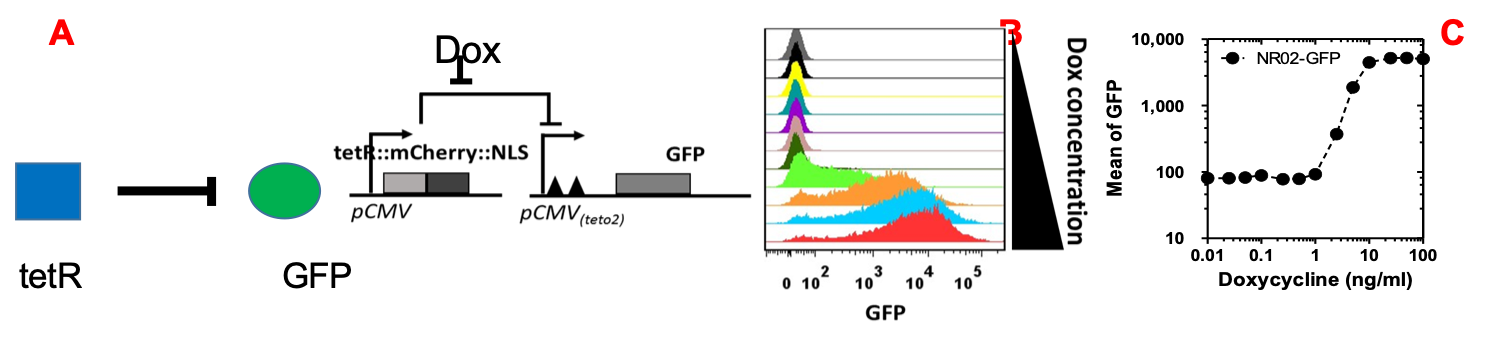
\includegraphics[width=1.0\linewidth]{Figures/part1.png}
\caption{Pictures of part 1}
\label{part_1_qestion_figure}
\end{figure}
%----------------------------------------------------------------------------------------

\section{Write step-by-step reactions}



\subsection{Symbols}

\begin{table}[H]
\caption{The symbols used in the model of doxycycline-induced GFP expression systems without feedback}
\label{tab:part1_symbols}
\centering
\begin{tabular}{l l}
\toprule

\tabhead{Symbol} & \tabhead{Definition} \\
\midrule
$D$ & The doxycycline molecular\\
$R$ & The tetR molecular\\
$R^{2}_{i}$ &   % ${\rm R^{2}_{i}}$ 改成正常体
The tetR-dimer molecular binds with \keyword{i} doxycycline molecular \\
$R_{sum}$ & 
Including $R^{2}_{0},R^{2}_{1},R^{2}_{2},R$ \\
$O_{m}$ & 
The $tetO^{2}$ binding with m $R^{2}_{0}(m = 0, 1, 2)$\\
%\quad$O_{00}$ & 
%\quad Both two tetOs are free \\
%\quad$O_{10}$ & 
%\quad One tetO is free and another is occupied by $R^{2}_{1}$ \\
%\quad$O_{11}$ & 
%\quad Both two tetOs are occupied by $R^{2}_{1}$ \\
%\quad$O_{20}$ & 
%\quad One tetO is free and another is occupied by $R^{2}_{0}$ \\
%\quad$O_{21}$ & 
%\quad Two tetO are respectively occupied by a $R^{2}_{0}$ and a $R^{2}_{1}$\\
%\quad$O_{22}$ & 
%\quad Both two tetOs are occupied by $R^{2}_{0}$ \\
$O_{on}$ & 
The binding situation of $tetO^{2}$ that turn on the expression of GFP mRNA\\
$O_{sum}$ & 
Including $O_{0}, O_{1}, O_{2}$ \\
$G$ & 
GFP \\
$P$ & 
RNA polymerase \\
$K_{1}$ & 
Reaction equilibrium constant of $R^{2}_{0}$ formation from $R$\\
$K_{2}$ & 
Reaction equilibrium constant of $R^{2}_{1}$ formation from $R^{2}_{0}$\\
$\sigma_{1}$ & 
$K_{3} = \sigma_{1} K_{2}$, \\ &so $\sigma_{1}$ represent binding strengths relative to the tetR-dimer-$tetO^{2}$ strength \\
$K_{3}$ & 
Reaction equilibrium constant of $R^{2}_{2}$ formation from $R^{2}_{1}$\\
$K_{4}$ & 
Reaction equilibrium constant of $O_{1}$ formation from $O_{0}$\\
$\sigma_{2}$ & 
$K_{5} = \sigma_{2} K_{4}$, \\ &so $\sigma_{2}$ represent binding strengths relative to the tetR-dimer-doxycycline strength \\
$K_{5}$ & 
Reaction equilibrium constant of $O_{2}$ formation from $O_{1}$\\
$k_{t}$ & 
Reaction constant of GFP production\\
$k_{d}$ & 
Reaction constant of protein degradation\\
$P_{0}$ & 
I assume that the concentration of $P$ remains constant as $P_{0}$ during time\\
$n$ & 
The number of proteins per mRNA transcript\\
$r$ & 
The basal rate of production of GFP\\
\bottomrule\\
\end{tabular}
\end{table}
\newpage

\subsection{Model}
The chemical reactions describing the network are naturally divided into two categories—fast and slow. The fast reactions have rate constants of order seconds and are therefore assumed to be in equilibrium with respect to the slow reactions, which are described by rates of order minutes.

Considering the reactions between tetR molecular, tetR-dimer molecular and doxycycline molecular, then we may write the equilibrium fast reactions :

\begin{equation} 
\begin{aligned} 
\centering
% \underset{A}{B}
% \overset{…}{…}
2R         &\underset{}{\overset{K_1}{\rightleftharpoons}} R^2_0 \\ 
R^2_0 + D  &\underset{}{\overset{K_2}{\rightleftharpoons}} R^2_1 \\ 
R^2_1 + D  &\underset{}{\overset{K_3}{\rightleftharpoons}} R^2_2 \\  
\end{aligned} 
\end{equation}

Considering the reactions between tetR-dimer molecular and $tetO^{2}$, and it is assumed that the tetR-dimer binding with doxycycline molecular could not binding to $tetO^{2}$, then we may write the equilibrium fast reactions :

\begin{equation} 
\begin{aligned} 
\centering
% \underset{A}{B}
% \overset{…}{…}
O_0 + R^2_0  &\underset{}{\overset{K_4}{\rightleftharpoons}} O_1 \\ 
O_1 + R^2_0  &\underset{}{\overset{K_5}{\rightleftharpoons}} O_2 \\  
\end{aligned} 
\end{equation}

It is assumed that only $O_0$ can bind to $tetO^{2}$. \\
The slow reactions are transcription and degradation :

\begin{equation} 
\centering
\begin{aligned} 
% \underset{A}{B}
% \overset{…}{…}
\qquad \qquad \quad[O_{on}]    &= [O_0] \\
%\qquad \qquad \quad[O_{on}]    &= [O_0] + \frac{1}{2}[O_1] \\
\qquad \qquad \quad O_{on} + P &\underset{}{\overset{k_t}{\rightarrow}} 
O_{on} + P + nG \\ 
\qquad \qquad \quad G          &\underset{}{\overset{k_d}{\rightarrow}} 
\phi \\  
\end{aligned} 
\end{equation}
I consider the expression level of tetR in the cell is stable, so 
$R_{sum}$ = $2([R_0^2]+[R_1^2]+[R_2^2])+[R]$ is a constant value. Also, the number of $tetO^{2}$ is depended by the number of plasmids in the cell. So the number of $tetO^{2}$ is a constant, which means $O_{sum}$ = $[O_0]+[O_1]+[O_2]$ does not change in a specific cell.

\subsection{Reactions}

\begin{equation*} 
\begin{aligned} 
\centering
% \underset{A}{B}
% \overset{…}{…}
2R           &\underset{}{\overset{K_1}{\rightleftharpoons}} R^2_0 \\ 
R^2_0 + D    &\underset{}{\overset{K_2}{\rightleftharpoons}} R^2_1 \\ 
R^2_1 + D    &\underset{}{\overset{K_3}{\rightleftharpoons}} R^2_2 \\  
O_0 + R^2_0  &\underset{}{\overset{K_4}{\rightleftharpoons}} O_1 \\ 
O_1 + R^2_0  &\underset{}{\overset{K_5}{\rightleftharpoons}} O_2 \\ 
[O_{on}]     &= [O_0] \\
%[O_{on}]     &= [O_0] + \frac{1}{2}[O_1] \\
O_{on} + P   &\underset{}{\overset{k_t}{\rightarrow}} O_{on} + P + nG \\ 
G            &\underset{}{\overset{k_d}{\rightarrow}} \phi \\  
\end{aligned} 
\end{equation*}

%----------------------------------------------------------------------------------------
%\newpage
\section{Write ODE equations from reactions}

Form the reactions above, ODE equations could be written and we know that : 
\begin{equation} 
\begin{aligned} 
\centering
% \underset{A}{B}
% \overset{…}{…}
K_i &= \frac{k_i}{k_{-i}}(i = 1,2,3,4,5) \\
\frac{d[R]}{dt} &= 2k_{-1}[R_0^2] - 2k_1 [R]^2  \\
\frac{d[R_0^2]}{dt} &= k_1 [R]^2 + k_{-2} [R^2_1] + k_{-4}[O_1] + k_{-5}[O_2] \\
				&\qquad - (k_{-1}+k_2[D]+k_4[O_0]+k_5[O_1]) [R_0^2] \\
\frac{d[R_1^2]}{dt} &= k_{-3}[R_2^2]-k_3[R^2_1][D]+k_2[R^2_0][D]-k_{-2}[R^2_1] \\
\frac{d[R_2^2]}{dt} &= k_{3}[R_2^1][D]- k_{-3}[R^2_2] \\
\frac{d[O_0]}{dt} &= k_{-4}[O_1]-k_4[O_0][R_0^2] \\
\frac{d[O_1]}{dt} &= k_4[O_0][R_0^2]-k_{-4}[O_1]+k_{-5}[O_2]-k_5[O_1][R_0^2] \\
\frac{d[O_2]}{dt} &= k_5[O_1][R_0^2]-k_{-5}[O_2] \\
\frac{d[G]}{dt} &= n k_t P_0 [O_0] - k_d[G] + r \\
%[O_{on}]     &= [O_0] \\
%[O_{on}]     &= [O_0] + \frac{1}{2}[O_1] \\
\end{aligned} 
\end{equation}
 


%----------------------------------------------------------------------------------------
\newpage
\section{Simplified the model with quasi-steady state assumption and justified the assumptions}

\subsection{Simplification}
Reaction in Eq.1.1 and Eq.1.2 can be simplified as steady-state.
So I get the equations :

\begin{equation} 
\begin{aligned} 
\centering
% \underset{A}{B}
% \overset{…}{…}
[R^2_0] &= K_1[R]^2 \\
[R^2_1] &= K_2[D][R^2_0] \\
[R^2_2] &= K_3[D][R^2_1] \\
[O_1]   &= K_4[R^2_0][O_0] \\
[O_2]   &= K_5[R^2_0][O_1] \\
R_{sum} &= 2([R_0^2]+[R_1^2]+[R_2^2])+[R] \\
O_{sum} &= [O_0]+[O_1]+[O_2] \\
K_{3} &= \sigma_{1} K_{2} \\
K_{5} &= \sigma_{2} K_{4} \\
\end{aligned} 
\end{equation}


Considering that the formation of tetR-dimer is very fast, which means that the value of $K_1$ is large and $[R]$ is very small, we can have:

\begin{equation} 
\begin{aligned} 
\centering
% \underset{A}{B}
% \overset{…}{…}
R_{sum} &= [R_0^2]+[R_1^2]+[R_2^2] \\
\end{aligned} 
\end{equation}

Then these equations could be written as:
\begin{equation} 
\begin{aligned} 
\centering
% \underset{A}{B}
% \overset{…}{…}
[R^2_1] &= K_2[D][R^2_0] \\
[R^2_2] &= \sigma_{1}K_2^2[D]^2[R^2_0] \\
[O_1]   &= K_4[R^2_0][O_0] \\
[O_2]   &= \sigma_{2}K_4^2[R^2_0]^2[O_0] \\
R_{sum} &= [R_0^2]+[R_1^2]+[R_2^2] \\
O_{sum} &= [O_0]+[O_1]+[O_2] \\
\end{aligned} 
\end{equation}

From Eq.1.3 we can get an ODE equation : 

\begin{equation*} 
\begin{aligned} 
\centering
% \underset{A}{B}
% \overset{…}{…}
\frac{d[G]}{dt} &= n k_t P_0 [O_0] - k_d[G] + r\\
\end{aligned} 
\end{equation*}

\newpage
Let $\alpha=nk_tP_0O_{sum}$, $\beta=K_4R_{sum}$, $y=[G]$, $x=[D]$, $N=K_2[D]$, 
$M=\beta[R^2_0]$ \\ then :

\begin{equation} 
\begin{aligned} 
\centering
% \underset{A}{B}
% \overset{…}{…}
\frac{dy}{dt} &= 
\frac{\alpha}{1+M+\sigma_{2}M^2} - k_dy + r\\
M &= 
\frac{\beta}{1+N+\sigma_{1}N^2}\\
N &= 
K_2x \\
\end{aligned} 
\end{equation}
%----------------------------------------------------------------------------------------

\section{Play with the parameters to mimic data from Figure \ref{part_1_qestion_figure} C}

\begin{figure}[H]
\centering
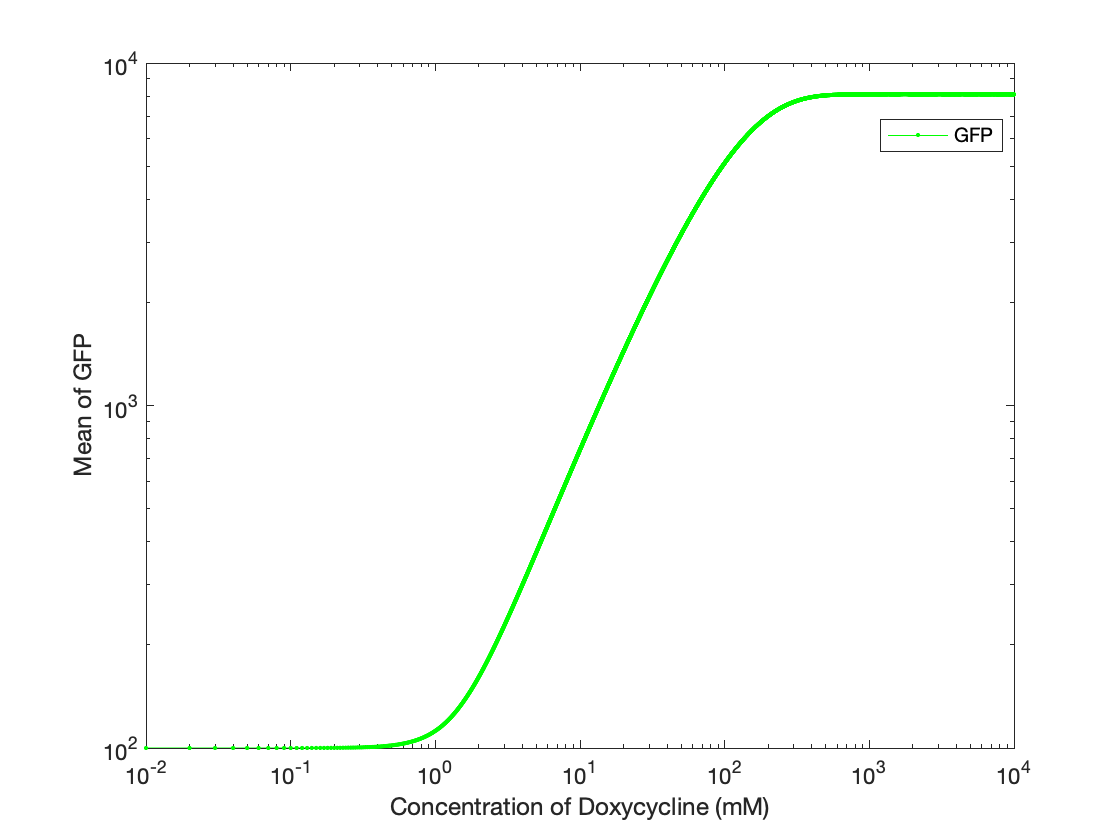
\includegraphics[width=1.0\linewidth]{Figures/Q1_1.png}
\caption{The modeling results for GFP with no feedback}
\label{part_1_model}
\end{figure}

$$K_2 = 100 mM^{-1}; \sigma_1 = 0.5; \beta = 10000 ; \sigma_2 = 0.5;$$ 
$$\alpha = 80 ; kd = 0.01h^{-1} ; r = 1mM*h^{-1} ;y_0 = 100mM$$

%----------------------------------------------------------------------------------------




%The \code{biblatex} package is used to format the bibliography and inserts references such as this one \parencite{Reference1}. The options used in the \file{main.tex} file mean that the in-text citations of references are formatted with the author(s) listed with the date of the publication. Multiple references are separated by semicolons (e.g. \parencite{Reference2, Reference1}) and references with more than three authors only show the first author with \emph{et al.} indicating there are more authors (e.g. \parencite{Reference3}). This is done automatically for you. To see how you use references, have a look at the \file{Chapter1.tex} source file. Many reference managers allow you to simply drag the reference into the document as you type.

